\documentclass[a4paper,11pt]{article}
\pdfoutput=1 % if your are submitting a pdflatex (i.e. if you have
             % images in pdf, png or jpg format)

\usepackage{jheppub} % for details on the use of the package, please
                     % see the JHEP-author-manual

\usepackage[T1]{fontenc} % if needed

%====================
\usepackage{url}
%\usepackage{minted}
\usepackage{setspace}
%\usemintedstyle{monokai}
\usepackage{amsmath}
\usepackage{fancyvrb}
\usepackage{graphicx} 
\usepackage{wrapfig} 
\usepackage{subcaption}
\graphicspath{ {images/} }
\usepackage{keyval}
\usepackage{braket}
\usepackage{amsthm}
\usepackage{hyperref}
\usepackage{indentfirst}
\setlength{\parindent}{22pt} 
\setlength{\parskip}{.5em} 
\usepackage{xcolor}
\hypersetup{
	colorlinks,
	linkcolor={red!50!black},
	citecolor={blue!50!black},
	urlcolor={blue!80!black}
}
%\renewcommand{\abstractname}{摘要} 
%\renewcommand{\figurename}{图}
%\renewcommand{\tablename}{表} 
%\renewcommand{\contentsname}{目录}
%\renewcommand{\refname}{参考文献}
\renewcommand{\acknowledgments}{\textbf{Prelude and acknowledgments}}
\setcounter{tocdepth}{3}

%====================

\theoremstyle{remark}
\newtheorem{remark}{Remark}[section]
\theoremstyle{defn}
\newtheorem{defn}{Definition}[section]

\title{\boldmath The $\mathcal{SO}(4)$ Symmetry of the Hydrogen Atom}


%% %simple case: 2 authors, same institution
%% \author{A. Uthor}
%% \author{and A. Nother Author}
%% \affiliation{Institution,\\Address, Country}

% more complex case: 4 authors, 3 institutions, 2 footnotes
\author{Naichao Hu}


% The "\note" macro will give a warning: "Ignoring empty anchor..."
% you can safely ignore it.

\affiliation{Department of Physics,\\Sun Yat-sen University}


% e-mail addresses: one for each author, in the same order as the authors
\emailAdd{hunch@mail2.sysu.edu.cn}


\abstract{We introduce some basic concepts in algebraic group theory and 
review the ``hidden'' $\mathcal{SO}(4)$ symmetry of the bound 
hydrogen atom in non-relativistic quantum mechanics, using an analogue of classical
Runge-Lenz vector and basic Lie group theory. 
This algebraic approach leads to a mathematical description of a higher dimension 
rotational symmetry for hydrogen atom. We examine also the entire energy spectrum
of the hydrogen atom.}


\begin{document} 
\maketitle
\flushbottom


\clearpage

\acknowledgments
\par
This note grows out of an assignment on solving hydrogen model from Prof Zwiebach's lectures
\footnote{See \url{http://ocw.mit.edu/courses/physics/8-05-quantum-physics-ii-fall-2013/index.htm}.}. I expand the material with more Lie group details and deform the method more
group theoretical guided.\par 
%Later I was able to expand the discussion on the dynamical symmetries in quantum mechanics 
%by including 3D harmonic oscillator model and putting more group theoretic material into %the note.\par
Though the detailed mathematics is first performed explicitly in the note, 
the methods in the note are far from original. They borrow heavily both from the books 
and the online resources listed below. 
\begin{itemize}
\item Zwiebach, Barton. \textit{Lecture notes}.
\item Townsend, John S. \textit{A modern approach to quantum mechanics}. University Science Books, 2000.
\item Schiff, Leonard I. \textit{Quantum mechanics}. McGraw-Hill, 1968.
\item Weinberg, Steven. \textit{Lectures on quantum mechanics}. Cambridge University Press, 2012.
\end{itemize}
\par Also, please note that for the derivation, there is a known explicit computing in
the book
\begin{itemize}
\item Greiner, Walter, and Berndt M\"uller. \textit{Quantum mechanics: symmetries}. Springer Science \& Business Media, 2012,
\end{itemize}
starting from p.460. But in the note, we take a different approach mentioned in Prof Zwiebach's lecture notes, motivated by more insight into the degeneracy of energy levels.
\clearpage

\section{Introduction}
\label{s:math}
%Symmetry 
Symmetric objects are so singular in the natural world that physicists must have
noticed them very early. Infinite models are constructed with the help of symmetry. 
In modern physics, for instance, we rely heavily on the Lagrangian/Hamiltonian, which is 
``the most general one that is invariant under some symmetries''
\footnote{By Yuval Grossman (Cornell) in Theoretical Concepts in Particle Physics, CERN Summer Student Lectures 2015.}.
This comment can be most easily in band theory, where we literally write down effective Hamiltonians 
from only the constraint of representations the bands follow. As another example, the celebrated
eight-fold way in particle physics is conceived with $\mathcal{SU}(3)$ group in mind.\par 

\begin{figure}[h!]
\centering
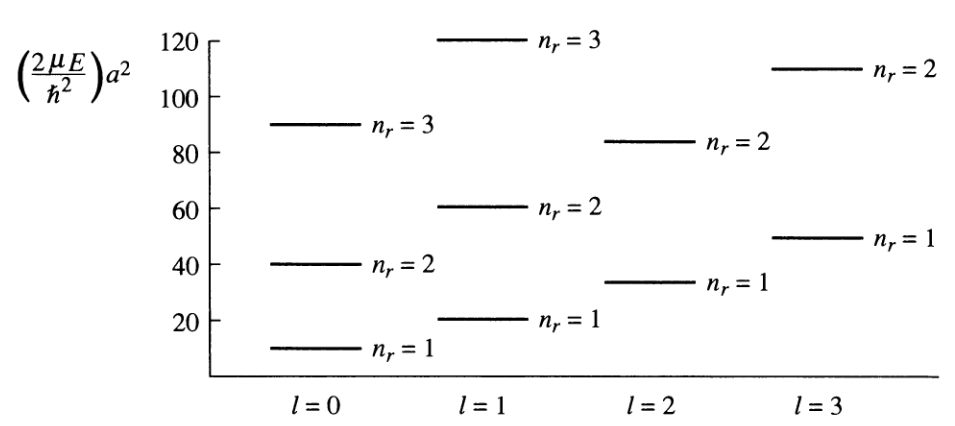
\includegraphics[width=\linewidth]{well}
\caption{Numerically calculated energy levels of the hydrogen atom (from \textit{Townsend}). 
Each line segment stands for a degeneracy of $2\ell+1$. Note that no manifest degeneracy for different $\ell$.}
\label{fig:well}
\end{figure}
Indeed, all symmetries simplifies problem if properly observed, but in physics mostly the need for a group theoretic approach
is in the case of dynamical symmetry instead of geometrical symmetry. This is due to that the geometry meets the eye is 
more or less simple and not very physical, while the dynamical symmetry or ``hidden symmetry'', normally hinted by unusual
properties, gives more insight to the problem. For example, in quantum mechanics, there is an utmost geometrical
symmetric object, the infinite spherical well. 
The potential is of a nice form 
\begin{equation}
V(r) = 
\left \{
  \begin{tabular}{ccc}
  0 &  & r<a, \\
  $\infty$ &  & r>a.
  \end{tabular}
\right.
\end{equation}
The solution to the problem is boring. We plot the energy levels of the infinite spherical well. Note that 
no interesting degeneracy arise.\par 
The dynamical symmetry we introduce in this note, on the other hand, contains more surprising degeneracies.
In classical mechanics, the the Kepler orbits are closed, which suggests there are more constants of
motion other than the orbital angular momentum. The new conserved quantity together with angular momentum
generates the $\mathcal{SO}(4)$ Lie groups. They are not geometrical but the symmetries in the phase
space, hence the name. These symmetries lead to an algebraic approach to determine the energy
levels.

\subsection{Some definitions}
Since we should be using jargon from group theory, we give a minimum set of concepts for readers not familiar with the topic to proceed.
\begin{defn}
A \textbf{group} is a non-empty set $\mathcal{G}$ with a binary operation $\oplus: \mathcal{G} \times \mathcal{G} \rightarrow \mathcal{G}$
satisfying the following three properties:
\begin{enumerate}
\item (associativity) for all $g,h,f \in \mathcal{G},\, (g \oplus h) \oplus f = g \oplus (h \oplus f)$,
\item (identity) there exists $e \in \mathcal{G}$ such that for all $g \in \mathcal{G}, \,g \oplus e = e \oplus g = g$,
\item (inverses) for all $g \in \mathcal{G}$, there exists $h \in \mathcal{G}$ such that $g \oplus h = h \oplus g = e$.
\end{enumerate}
\end{defn}
The \textbf{rank} of a finitely generated group $\mathcal{G}$ can be understood as the maximum number of mutually commuting generators.
\begin{defn}
A \textbf{Casimir operator} in a Lie group is a invariant bilinear form that commutes with every generators of the group.
\end{defn}
A prototypical example is the squared angular momentum operator $\textbf{J}^2$, which is a Casimir element of the three-dimensional rotation group.\par
We also introduce the Lie groups we 'll use in a moment. All $n\times n$ unitary matrix forms the group $\mathcal{U}(n)$.
Evidently the group has $n^2$ independent parameters. 
If we require the determinant of the matrices to be equal to $+ 1$, the
new group is called $\mathcal{SU}(n)$, characterized by $n^2-1$ parameters. 
If we further require all matrices are real and orthonormal to each other, with determinant equal to unity, we obtain $\mathcal{SO}(n)$. 
The generators of any Lie group are defined in terms of the group
elements that are infinitesimally close to the unit element. Thus, if the group has $n$ parameters, the $n$ generators 
specify an infinitesimal element of the group in terms of $n$ infinitesimal real parameters.

\section{Dynamical symmetries and degeneracy}
The hydrogen atom is the very first model physicists can solve even before Schr\"odinger wrote down his equation. 
The method we introduce here was first proposed by Pauli (\textit{Zs. f. Phys. 36, 336 (1926)}), 
and it utilizes more symmetry then a quantum mechanic 
textbook usually do. The method, in my opinion, reveals more physics than solving a partial differential equation,
albeit it can't give more than the energy levels.\par 

\subsection{Background}
The Hamiltonian for a hydrogen atom is 
\begin{equation}
H = \frac{p^2}{2m}-\frac{e^2}{r}.
\end{equation}
Following the standard procedure and solving the radial equation gives a quantized energy
\begin{equation}
\label{eq:elevel}
E_n = -\frac{me^4}{2\hbar^2n^2} = -\frac{me^4}{2\hbar^2(n_r+\ell+1)^2} = \frac{\alpha^2mc^2}{2n^2},
\end{equation}
where $n=n_r+\ell+1$ is the principle quantum number, $\alpha = e^2/\hbar c\sim1/137$ the fine-structure number.
Note that $\alpha^2\sim 5.33\times 10^{-5}$. Since the spin-orbit coupling has a characteristic energy of 
$\sim \alpha^4mc^2$, the hyperfine spliting $\sim (m_e/m_p) \alpha^4mc^2$, we can safely ignore these effects here.
From eq.~\eqref{eq:elevel} we can infer the degeneracy of $E_n$ to be 
\begin{equation}
\sum_{\ell=0}^{n-1}(2\ell+1) = n^2.
\end{equation}
\par
To have a better understanding, we can plot this (indeed) fancy degeneracy in the left panel of fig.~\ref{fig:hydrogen}.
However, the derivation in most textbooks won't disclose why physically this is true.
\begin{figure}
\centering
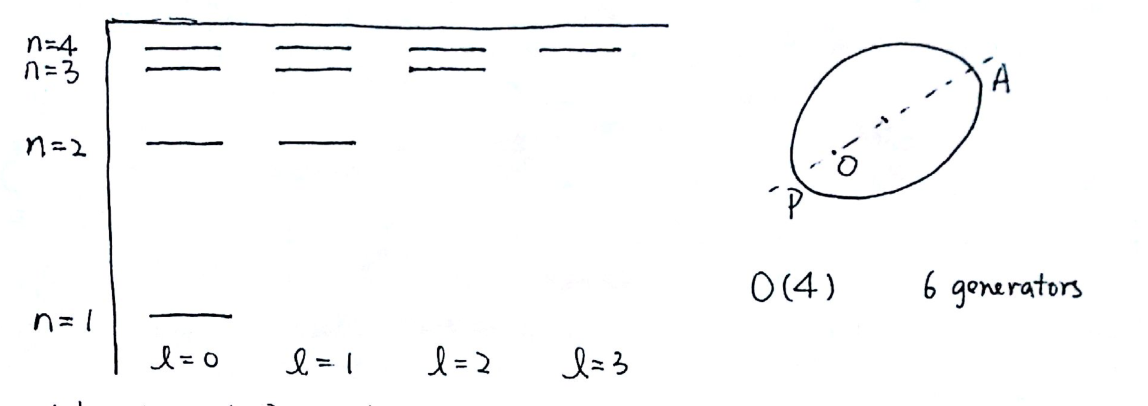
\includegraphics[width=\linewidth]{hydrogen}
\caption{Left panel: the energy levels of the hydrogen atom. Each line segment stands for a degeneracy of $2\ell+1$. 
Right panel: a schematic trace of a particle under the force of an inverse-square central type. O is one of the focuses.}
\label{fig:hydrogen}
\end{figure}

\subsection{Classical Runge-Lenz vector}
As others, our method also borrow quantities to understand these ``incidents''. From classical mechanics, we understand for 
Kepler type orbits, the conservation of $H$ and $\vec{L}$ is not enough to keep the orbit closed. 
A small deviation of the potential, e.g. general relativity effect for the Mercury, induces a slow procession. 
To have a closed orbit like the right panel of fig.~\ref{fig:hydrogen}, we need another constant of motion to characterize 
the orientation of the major axis in orbital plane. Such a vector is known as the Runge-Lenz vector, but first found by Laplace:
\begin{equation}
\vec{R} = \frac{\vec{p}\times\vec{L}}{m}-\frac{e^2}{r}\vec{r}. 
\end{equation}
It's easy to check the Runge-Lenz vector has the following properties.
\begin{align}
&\frac{d}{dt}\vec{R} = 0, \label{eq:pp1} \\
&|\vec{R}|^2 = \frac{2H}{m}\vec{L}^2+e^4, \label{eq:pp2} \\
&\vec{L}\cdot\vec{R} = 0. \label{eq:pp3}
\end{align}
For the elliptical orbit of a classical particle, the Runge-Lenz vector $\vec{R}$ in fact points
into the direction of the semi major axis of the ellipse, while the length of it is the eccentricity.

\subsection{Runge-Lenz operator}
To translate the vector to quantum mechanics, we must first promote everything to operator and 
hermitianizing the Runge-Lenz operator, i.e.
\begin{equation}
\begin{split}
\hat{R} &= \frac{1}{2}(\vec{R}+\vec{R}^{\dagger})\\
&= \frac{1}{2m}(\vec{p}\times\vec{L}-\vec{L}\times\vec{p})-\frac{e^2}{r}\vec{r}\\
&= \frac{1}{m}(\vec{p}\times\vec{L}-i\hbar \vec{p})-\frac{e^2}{r}\vec{r}.
\end{split}
\end{equation}
\par Now we need to check if properties ~\eqref{eq:pp1}-~\eqref{eq:pp3} remians true. \par
For eq.~\eqref{eq:pp1}, we now need to prove $[\hat{R},\hat{H}]=0$. For simplicity, we denote $f=e^2/r$.
Then $\hat{H} = \hat{p}^2/2m-f,\,\hat{R} = \frac{1}{m}(\vec{p}\times\vec{L}-i\hbar \vec{p})-f\vec{r}$. 
With some careful calculations, we find
\begin{align}
[\hat{p}^2,f\vec{r}] &= \frac{\hbar}{i}[(\hat{p}\hat{r})\hat{r}\frac{f'}{r}+\frac{f'}{r}\hat{r}(\hat{r}\hat{p})+\hat{p}f+f\hat{p}],\\ 
[\hat{p}\times\hat{L}-\hat{L}\times\hat{p},f] &=
\frac{\hbar}{i}[(\hat{p}\hat{r})\hat{r}\frac{f'}{r}+\frac{f'}{r}\hat{r}(\hat{r}\hat{p})-\hat{p}rf'-rf'\hat{p}],
\end{align}
where $f' := \frac{d}{dr} = -f/r$. It's now evident that 
\begin{equation}
\begin{split}
[\hat{H},\hat{R}] &=  -\frac{\hbar}{2mi}[\hat{p}(f+rf')+(f+rf')\hat{p}]\\
&=0.
\end{split}
\end{equation}
\par Then we calculate the length-squared of the quantum Runge-Lenz vector. We first note the following equations always hold true.
\begin{align}
&(\hat{L}\times\hat{p})\hat{r} = -\hat{L}^2, \label{eq:1} \\
&i\hbar(\hat{p}\frac{\hat{r}}{r} - \frac{\hat{r}}{r}\hat{p}) = \frac{2\hbar^2}{r}, \label{eq:t2} \\
&(\hat{L}\times\hat{p})(\hat{p}\times\hat{L}) = -\hat{p}^2\hat{L}^2. \label{eq:t3}
\end{align}
Now we can proceed further
\begin{equation}
\begin{split}
\hat{R}^2 
&=[\frac{1}{m}(-\hat{L}\times\hat{p}+i\hbar\hat{p})-\frac{e^2}{r}\hat{r}]
[\frac{1}{m}(\hat{p}\times\hat{L}-i\hbar\hat{p})-\frac{e^2}{r}\hat{r}]\\
&=\frac{1}{m^2}[-(\hat{L}\times\hat{p})(\hat{p}\times\hat{L}) + i\hbar(\hat{L}\times\hat{p})\hat{p} + i\hbar\hat{p}(\hat{p}\times\hat{L}) + \hbar^2\hat{p}^2]
 -\frac{e^2}{m}[(-\hat{L}\times\hat{p}+i\hbar\hat{p})\frac{\hat{r}}{r} \\
 &\quad + \frac{\hat{r}}{r}(\hat{p}\times\hat{L}-i\hbar\hat{p})]+e^4\\
&=\frac{1}{m^2}(\hat{p}^2\hat{L}^2+\hbar^2\hat{p}^2)-\frac{e^2}{m}(\frac{2\hat{L}^2}{r}+\frac{2\hbar^2}{r})+e^4\\
&=e^4+\frac{2\hat{H}}{m}(\hat{L}^2+\hbar^2).
\end{split}
\end{equation}
Note the resemblance to the classical result!\par 
We then continue to property eq.~\eqref{eq:pp3}. One can easily check that $\hat{L}\hat{R}=\hat{R}\hat{L}=0$.
But the full quantum analogy is the commutation relations between $\hat{L}$ and $\hat{R}$, i.e.
\begin{align}
[L_i,L_j]&=i\hbar\epsilon_{ijk}L_k   &  [R_i,L_i]&=0\\
[R_i,L_j]&=i\hbar\epsilon_{ijk}R_k   &  [R_i,R_j]&=-\frac{2\hat{H}}{m}i\hbar\epsilon_{ijk}L_k.
\end{align}
The first three are easy to check by definition, while the fourth is rather tricky. We note that it's equivalent to 
\begin{equation}
(\hat{R}\times\hat{R})_i = -\frac{2\hat{H}}{m}i\hbar\epsilon_{ijk}r_jp_k.
\end{equation}
\par The calculation is actually so involved that \textit{Weinberg} referred to as tedious. Here we simplify the progress by a 
trick given by Schwinger. First, we make the insight that for any to conserved operators $S_1$ and $S_2$, their commutation must
also be conserved due to the Jacobi identity
\begin{equation}
[[S_1,S_2],H]+[[H,S_1],S_2]+[[S_2,H],S_1]=0.
\end{equation}
So $[R_i,R_j]$ is a conserved object. And our options are $\hat{L},\,\hat{R}$ and $\hat{L}\times\hat{R}$.
We narrow the options down by perform the parity operator: $\mathcal{P}\hat{r}=-\hat{r}$. Since
\begin{align}
\mathcal{P}\hat{p} &= -\hat{p} & \mathcal{P}\hat{L} &= \hat{L} & \mathcal{P}\hat{R} &= -\hat{R},
\label{eq:parity}
\end{align}
the choice is $\hat{R}\times\hat{R} = \alpha\hat{L}$, where $\alpha$ is a constant we now determine.
\begin{equation}
\begin{split}
(\hat{R}\times\hat{R})_i 
&= \epsilon_{ijk}\left[\frac{1}{m}(\epsilon_{jmn}p_m\epsilon_{nab}r_ap_b-i\hbar p_j)-e^2\frac{r_j}{r}\right]
\left[\frac{1}{m}(\epsilon_{kmn}p_m\epsilon_{nab}r_ap_b-i\hbar p_k)-e^2\frac{r_k}{r}\right]\\
&= \epsilon_{ijk}\left[\frac{1}{m}\bigg(\hat{p}^2r_j-(\hat{p}\hat{r}+i\hbar) p_j\bigg)-e^2\frac{r_j}{r}\right]
\left[\frac{1}{m}\bigg(\hat{p}^2r_k-(\hat{p}\hat{r}+i\hbar) p_k\bigg)-e^2\frac{r_k}{r}\right]\\
&= \epsilon_{ijk}\left[\frac{1}{m^2}\bigg(-\hat{p}^2r_j(\hat{p}\hat{r}+i\hbar) p_k-(\hat{p}\hat{r}+i\hbar) p_j\hat{p}^2r_k\bigg)
+\frac{e^2}{m}\bigg(\frac{r_j}{r}(\hat{p}\hat{r}+i\hbar) p_k+(\hat{p}\hat{r}+i\hbar) p_j\frac{r_k}{r}\bigg)\right]\\
&= -\frac{2\hat{H}}{m}i\hbar\epsilon_{ijk}r_jp_k.
\end{split}
\end{equation}

\subsection{From 3D to 4D}
Since $\hat{H}$ is independent of time and commutes with both $\hat{L}$ and $\hat{R}$, we replace $\hat{H}$ with $E$ and define
\begin{equation}
\hat{R}':=\sqrt{-\frac{m}{2E}}\hat{R},
\end{equation}
which gives cleaner relations with $\hat{L}$ as 
\begin{equation}
[R'_i,R'_j]=i\hbar \epsilon_{ijk}L_k.
\end{equation}
We know $\hat{L}$ formed a closed algebra and corresponds to the group $\mathcal{SO}(3)$. With the help of the commutations, we
can show there is another closed algebra formed by $\hat{L}$ and $\hat{R}$. First we relabel $\hat{r},\,\hat{p},\,\hat{L}$ as
\begin{align}
\hat{r}&=(r_1,r_2,r_3) & \hat{p}&=(p_1,p_2,p_3) & \hat{L}&=(L_{23},L_{31},L_{12}),
\end{align}
and $\hat{R}'$ as 
\begin{equation}
\hat{R}' = (L_{14},L_{24},L_{34}).
\end{equation}
Note that if we write $L_{ij}:=r_ip_j-r_jp_i$ and let $[r_i,p_j]:=i\hbar \delta_{ij}$, we readily establish the full commutation 
relations between $\hat{L}$ and $\hat{R}'$. Thus even only formally, we generalized $\hat{L}$ from 3D to 4D. And the 6 generators
effectively generate the group $\mathcal{SO}(4)$.

\subsection{The group $\mathcal{SO}(4)$}
To better the understanding of the mass we performed, we interpret the result from another angle. It can be proved that there is a
homomorphism from the group $\mathcal{SO}(4)$ to $\mathcal{SO}(3)\otimes\mathcal{SO}(3)$, that is, two independent angular momentum
can be constructed.\par
Define
\begin{align}
\hat{I} &= \frac{1}{2}(\hat{L}+\hat{R}') & \hat{K} &=  \frac{1}{2}(\hat{L}-\hat{R}').
\end{align}
Their properties are as follows
\begin{align}
&[I_i,I_j] = i\hbar \epsilon_{ijk}I_k, & &[K_i,K_j] = i\hbar \epsilon_{ijk}K_k,\\
&[\hat{I},\hat{K}] = 0, & &[\hat{I},\hat{H}] = [\hat{K},\hat{H}] = 0.
\end{align}
Note that $\mathcal{SO}(4)$ is of rank 2, which gives two Casimir operators\footnote{It's defined that a Casimir operator of a group 
commutes with all generators of the group.}, i.e.
\begin{align}
\hat{I}^2 &= \frac{1}{4}(\hat{L}+\hat{R}')^2, & \hat{K}^2 &= \frac{1}{4}(\hat{L}-\hat{R}')^2.
\end{align}
The eigenvalues are
\begin{align}
&I^2 = i(i+1)\hbar^2, & &K^2 = k(k+1)\hbar^2, & &i,k=0,\frac{1}{2},1,\ldots.
\end{align}
Due to he cross term that vanishes as we have checked, $\hat{I}^2=\hat{K}^2$ and $i=k$.
A third operator is needed for the energy levels, that is, $\hat{C}:=(\hat{L}^2+\hat{R}'^2)/2 = \hat{I}^2+\hat{K}^2 = 2k(k+1)\hbar^2$,
$k=0,\frac{1}{2},1,\ldots$. On the other hand, 
\begin{equation}
\begin{split}
\hat{C} &= \frac{1}{2}(\hat{L}^2+\hat{R}'^2)\\
&= \frac{1}{2}(\hat{L}^2-\frac{m}{2E}\hat{R}^2)\\
&= \frac{me^4}{4E}-\frac{1}{2}\hbar^2.
\end{split}
\end{equation}
Thus 
\begin{equation}
E=-\frac{me^4}{2\hbar^2(2k+1)^2}.\label{eq:ele}
\end{equation}
We identify $n=2k+1$, hacing values $1,2,3,\ldots$. 
\par 
The reason we use half-integer values for $i,\,k$ is $\hat{L}=\hat{I}+\hat{K}$ and $i=k$. By the rules of addition 
of angular momentum, $\ell$ can take any value ranging from $i+k=2k=n-1$ to $|i-k|=0$, by integer steps. Or in 
representation language,
\begin{equation}
\textbf{$\frac{1}{2}$(n-1)}\otimes\textbf{$\frac{1}{2}$(n-1)} = 
\textbf{n-1}\oplus\textbf{n-2}\oplus\ldots\oplus\textbf{1}\oplus\textbf{0},
\end{equation}
which more naturally describe fig.~\ref{fig:hydrogen}. Thus the range of $\ell$ for a given $n$ is actually 
constrained by the physical restriction that it can only take integer values up to $n-1$.
\begin{remark}
We need to clarify that our considerations are only limited to bound states. For scattering states, $E>0$, $\hat{R}'$ need to be modified
to stay Hermitian. Then commutations are messed up. The parts from $\hat{I},\,\hat{K}$ would be invalid.
\end{remark}
\begin{remark}
There is yet another way to understand the degeneracy, from directly the group $\mathcal{SO}(4)$. More geometrical than physical. 
We do not discuss the method here. But for the intrigued, see Weinberg p.145.
\end{remark}

\subsection{3D isotropic harmonic oscillator}
Another interesting object we will not discuss in detail is the 3D isotropic harmonic oscillator, with
the symmetry of $\mathcal{SU}(3)$ type. Still we show the energy levels in fig.~\ref{fig:sho} for
another feature of hydrogen atom. One note that there is a very distinct property for the degeneracy
from fig.~\ref{fig:hydrogen}.\par  
\begin{figure}
\centering
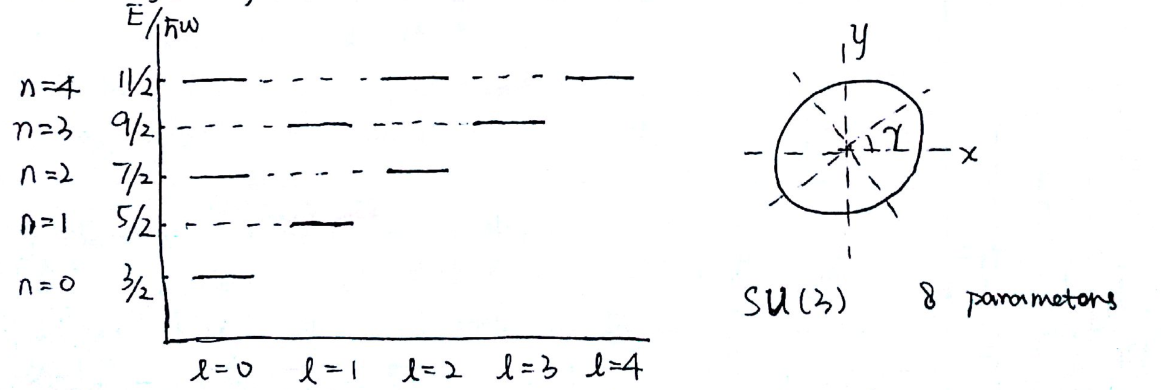
\includegraphics[width=\linewidth]{sho}
\caption{Left panel: the energy levels of the 3D isotropic harmonic oscillator. Each line segment stands for a degeneracy of $2\ell+1$. 
Right panel: a particular solution of the classical orbit problem is an ellipse
with semimajor axis a and semiminor axis b, which has its major axis
oriented so as to make an angle $\gamma$ with the x axis. Point of attraction is O.}
\label{fig:sho}
\end{figure}
That is, states of even and odd $l$ are degenerate in fig.~\ref{fig:hydrogen}, albeit $\hat{L}$ has
a well-defined parity as seen in eq.~\ref{eq:parity}.
The two generators case is the reason. Since $\hat{L}$ is axial and $\hat{R}$ polar, and the states are 
generated by both, they lost the well defined parity. In the harmonic oscillator case, there is only one 
generator presence, and states has a well-defined parity.

\section{Concluding remarks}
In conclusion, we can say that the bound states of the hydrogen atom can be determined
by the principal quantum number $n$, which takes the values $n = 1, 2,\ldots$. For
given $n$, we have $n^2$ states with angular momenta $\ell = 0, 1, \ldots , n-1$, and energy $E_n$
given by eq.~\eqref{eq:elevel}, or eq.~\eqref{eq:ele}.\par  
We finally remark that this symmetry is not limited to the problem discussed here, despite its antiquity. 
It can be more general, i.e. the n-dimensional hydrogen atom has the $\mathcal{SO}(n+1)$ and the isotropic oscillator has the $\mathcal{SU}(n)$ symmetry. And objects that shares the same symmetry can be analysed
much the same way.
\end{document}
